\documentclass[11pt]{article}
\usepackage{fullpage}
%\usepackage[top=2cm, bottom=2cm, left=3cm,right=2cm]{geometry}
\usepackage{amsfonts}
\usepackage{graphicx}

\def\eq1{y =\frac{x}{3x^2+x+1}}
\def\labelaxes{Remember to include a scale and label your axis.}

\begin{document}

The set of Natural numbers is denoted by $\mathbb{N}$.

The set of Integers is denoted by $\mathbb{Z}$.

The set of Real numbers is denoted by $\mathbb{R}$

Graph $\eq1$. \labelaxes

Identify the asymptotes for the graph of $\eq1$.

\begin{center}
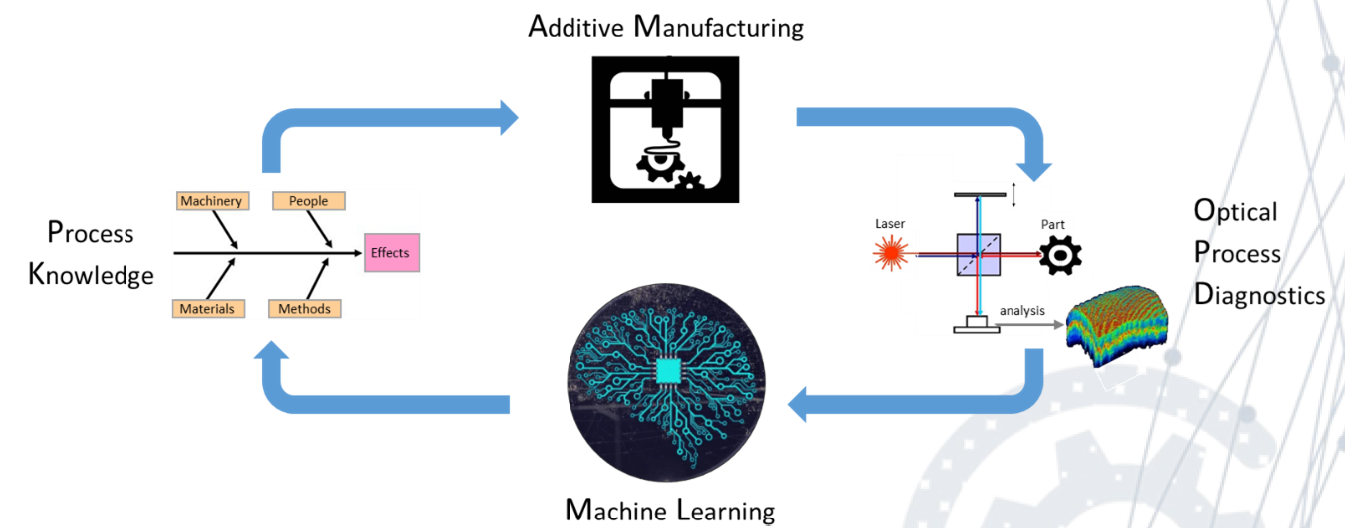
\includegraphics[scale=0.2]{DA.png}

Image must be save as .png, .jpg, .gif, .pdf file
\end{center}

\begin{enumerate}
\item Describe a real-world situation that could be represented by the equation $a=b+3$. Include a definition for each variable.
\item Explain the difference between $-3^2$ and $(-3)^2$ in terms of order of operations.

\end{enumerate}

\end{document}